
\documentclass{standalone}
\usepackage{pgf-umlcd}
\renewcommand{\unidirectionalAssociation}[4]
{
  \draw[umlcd style, ->] (#1) -- (#4)
  node[near end, auto]{#2}
  node[near end, auto,swap]{#3};
}
\begin{document}
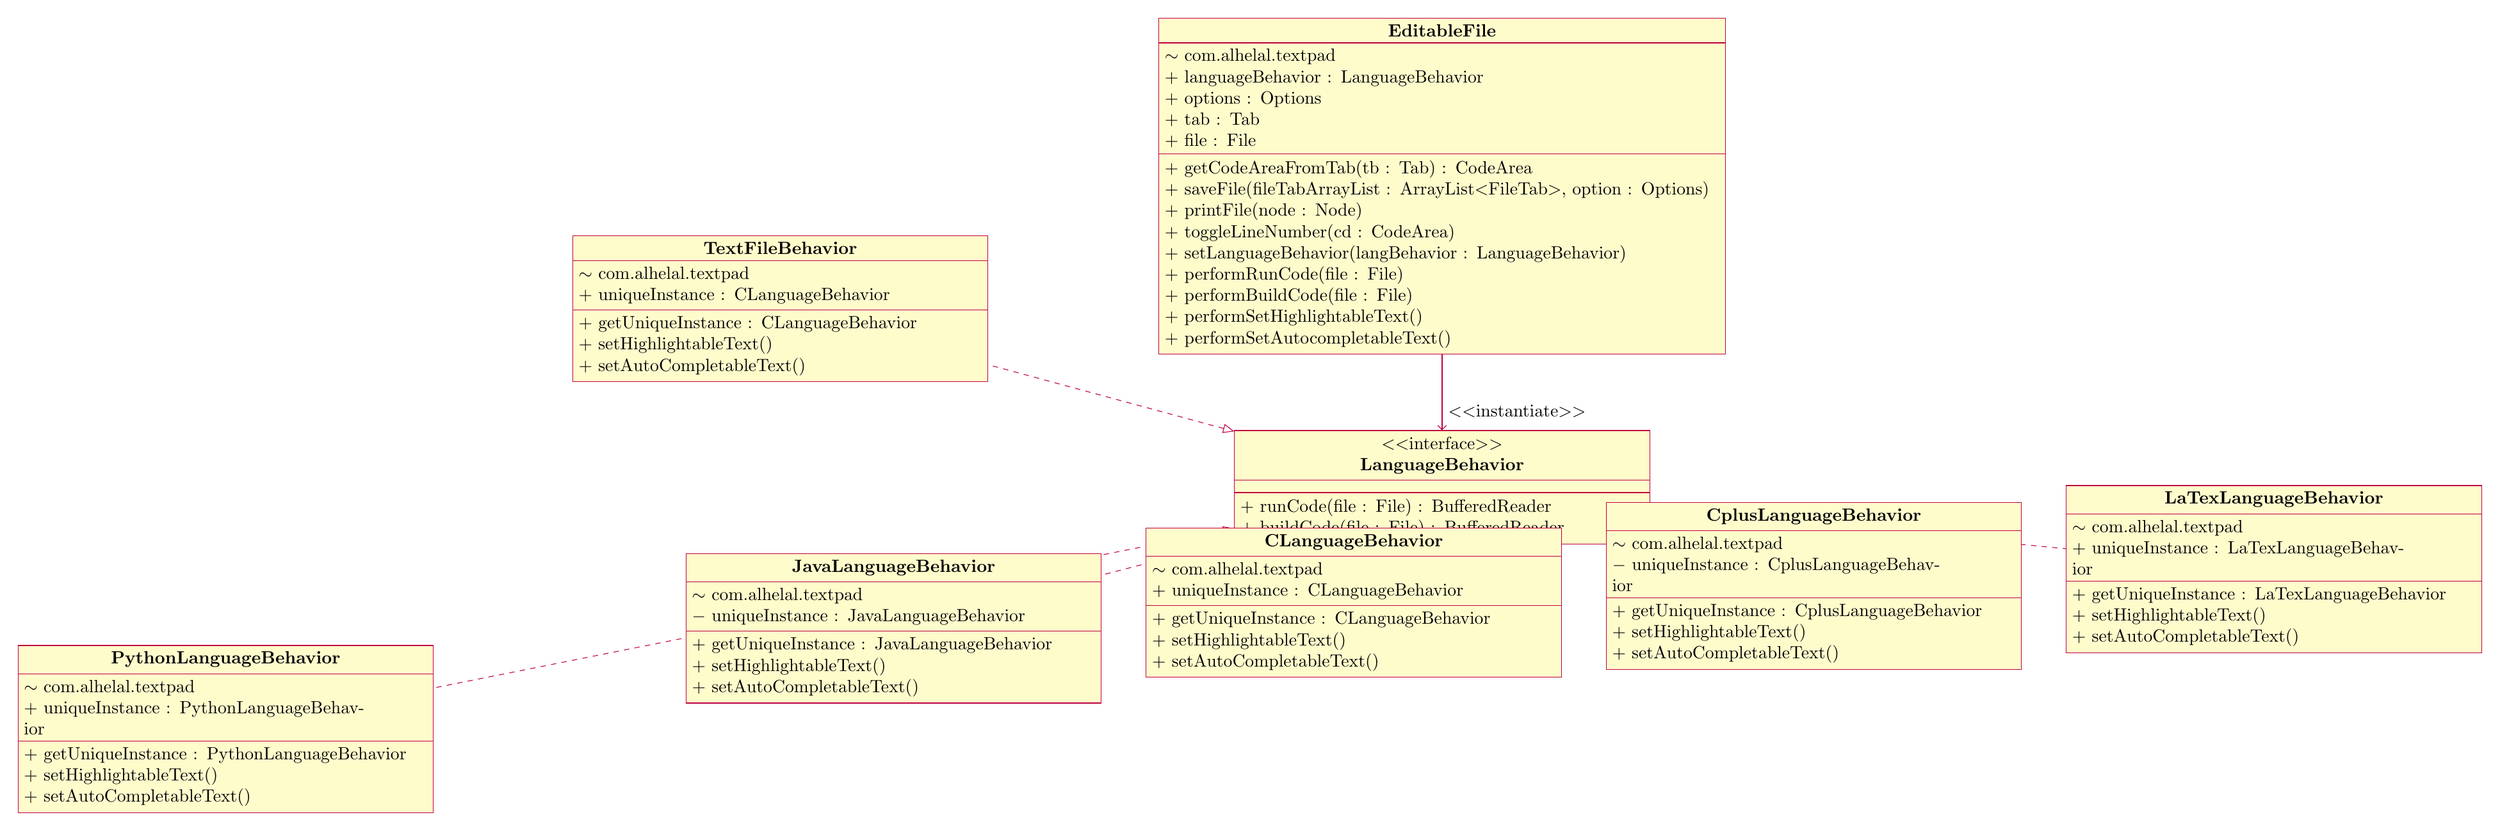
\begin{tikzpicture}
  \begin{class}[text width = 11cm,anchor=north west, xshift=6cm]{EditableFile}{0,0}
    \attribute{$\sim$ com.alhelal.textpad}
    \attribute{+ languageBehavior : LanguageBehavior} 
    \attribute{+ options : Options} 
    \attribute{+ tab : Tab}
    \attribute{+ file : File}
    \operation{+ getCodeAreaFromTab(tb : Tab) : CodeArea} 
    \operation{+ saveFile(fileTabArrayList : ArrayList$<$FileTab$>$, option : Options)}
    \operation{+ printFile(node : Node)}
    \operation{+ toggleLineNumber(cd : CodeArea)}
    \operation{+ setLanguageBehavior(langBehavior : LanguageBehavior)}
    \operation{+ performRunCode(file : File)}
    \operation{+ performBuildCode(file : File)}
    \operation{+ performSetHighlightableText()}
    \operation{+ performSetAutocompletableText()}
  \end{class}
  \begin{interface}[text width=8cm,yshift=-1.5cm]{LanguageBehavior}{EditableFile.south}
    \operation{+ runCode(file : File) : BufferedReader}
    \operation{+ buildCode(file : File) : BufferedReader}
  \end{interface}
%
  \begin{class}[text width = 8cm,yshift=-2cm,xshift=-20cm]{PythonLanguageBehavior}{LanguageBehavior.south west}
    \implement{LanguageBehavior}
    \attribute{$\sim$ com.alhelal.textpad}
    \attribute{+ uniqueInstance : PythonLanguageBehavior}
    \operation{+ getUniqueInstance : PythonLanguageBehavior}
    \operation{+ setHighlightableText()}
    \operation{+ setAutoCompletableText()}
  \end{class}
%
  \begin{class}[text width = 8cm,anchor=west,xshift=5cm,yshift=2cm]{JavaLanguageBehavior}{PythonLanguageBehavior.east}
    \implement{LanguageBehavior}
    \attribute{$\sim$ com.alhelal.textpad}
    \attribute{$-$ uniqueInstance : JavaLanguageBehavior}
    \operation{+ getUniqueInstance : JavaLanguageBehavior}
    \operation{+ setHighlightableText()}
    \operation{+ setAutoCompletableText()}
  \end{class}
%
  \begin{class}[text width = 8cm,xshift=5cm,yshift=2cm]{CLanguageBehavior}{JavaLanguageBehavior.east}
    \implement{LanguageBehavior}
    \attribute{$\sim$ com.alhelal.textpad}
    \attribute{+ uniqueInstance : CLanguageBehavior}
    \operation{+ getUniqueInstance : CLanguageBehavior}
    \operation{+ setHighlightableText()}
    \operation{+ setAutoCompletableText()}
  \end{class}

  \begin{class}[text width = 8cm,yshift=5cm,xshift=-9cm]{TextFileBehavior}{LanguageBehavior.west}
    \implement{LanguageBehavior}
    \attribute{$\sim$ com.alhelal.textpad}
    \attribute{+ uniqueInstance : CLanguageBehavior}
    \operation{+ getUniqueInstance : CLanguageBehavior}
    \operation{+ setHighlightableText()}
    \operation{+ setAutoCompletableText()}
  \end{class}
%
  \begin{class}[text width = 8cm,yshift=2cm, xshift=5cm]{CplusLanguageBehavior}{CLanguageBehavior.east}
    \implement{LanguageBehavior}
    \attribute{$\sim$ com.alhelal.textpad}
    \attribute{$-$ uniqueInstance : CplusLanguageBehavior}
    \operation{+ getUniqueInstance : CplusLanguageBehavior}
    \operation{+ setHighlightableText()}
    \operation{+ setAutoCompletableText()}
  \end{class}
%
%
  \begin{class}[text width = 8cm,yshift=2cm,xshift=5cm]{LaTexLanguageBehavior}{CplusLanguageBehavior.east}
    \implement{LanguageBehavior}
    \attribute{$\sim$ com.alhelal.textpad}
    \attribute{+ uniqueInstance : LaTexLanguageBehavior}
    \operation{+ getUniqueInstance : LaTexLanguageBehavior}
    \operation{+ setHighlightableText()}
    \operation{+ setAutoCompletableText()}
  \end{class}
  \unidirectionalAssociation{EditableFile}{$<<$instantiate$>>$}{}{LanguageBehavior}
\end{tikzpicture}
  \end{document}
